\section*{Problem 3}
My implementation of K-means starts with randomly assign K centroids.
Then for each pixel I found the eucleidian distance between the centers
and the pixel. Then I add the pixel to the Kth minimum distance element
in order after dividing this with the number of points on this cluster to
get the new center. The code can be found in problem3.m. It has as an
argument the number of clusters it should produce. It returns the number
of clusters with at least a pixel in.
\begin{figure}[ht] 
  \begin{subfigure}[b]{0.5\linewidth}
    \centering
    
\includegraphics[width=0.75\linewidth]{figures/initial.png}
    \caption{Initial image} 
    \vspace{4ex}
  \end{subfigure}%% 
  \begin{subfigure}[b]{0.5\linewidth}
    \centering
    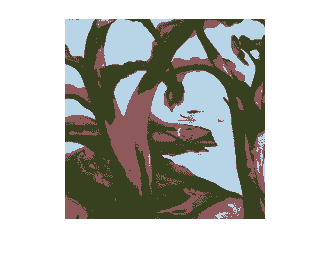
\includegraphics[width=0.75\linewidth]{figures/kmeans3.png} 
    \caption{K=3 clusters}
    \vspace{4ex}
  \end{subfigure} 
  \begin{subfigure}[b]{0.5\linewidth}
    \centering
    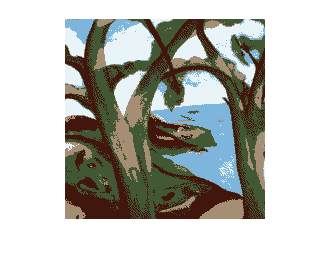
\includegraphics[width=0.75\linewidth]{figures/kmeans5.png}
    \caption{K=5 clusters} 
  \end{subfigure}%%
  \begin{subfigure}[b]{0.5\linewidth}
    \centering
    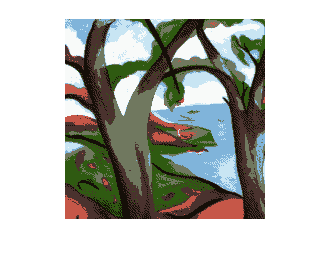
\includegraphics[width=0.75\linewidth]{figures/kmeans8.png} 
    \caption{K=8 clusters} 
  \end{subfigure} 
  \caption{Illustration of various K-means clustering}
\end{figure}

For the initialization and inconsistencies:
Picking random points as initialization points can lead to empty or weird clusters. Specifying
more clusters as you can handle can create empty ones (if you run my program with 20 you will get
only 17 clusters) or the ones that will be created are not distinct. Picking pixels form the image
can lead to inconsistencies also as you may pick an outlier that will not have any point as cluster.
Also picking some specific ones (I had done some experiments with 3 clusters(Red, Green, Blue) or 5
(the previous plus Black and White)) but I did not had any better result. 

In order to solve this problem the community chooses either to run multiple time the K-means and
pick the best. But still this technique is not guaranteed. Other are running other cluster algorithms
like hierarchical in order to get some good initial points. Another solution is to remove outliers
in order to pick some more consistent centroids. A wide applicable approach as the problem is NP-hard
is the K-means++ algorithm. Matlab's kmeans function is using the k-meams++ algorithm.
